\documentclass[10pt,twocolumn,letterpaper]{article}
\usepackage[pagenumbers]{cvpr}

\usepackage{amsthm}
\usepackage{tikz}
\usetikzlibrary{arrows.meta,positioning,calc}

\definecolor{cvprblue}{rgb}{0.21,0.49,0.74}
\usepackage[breaklinks,colorlinks,allcolors=cvprblue]{hyperref}

\graphicspath{{../results/plots/24_paper_20261031/}}

\theoremstyle{plain}
\newtheorem{proposition}{Proposition}
\AtBeginDocument{\crefname{proposition}{Prop.}{Props.}}

\newcommand{\Ang}{\,\AA}
\newcommand{\logT}{\ensuremath{\log T}}
\newcommand{\mudrop}{\ensuremath{\mu_{\mathrm{drop}}}}
\DeclareMathOperator*{\argmin}{arg\,min}

\def\confName{CVPR}
\def\confYear{2027}

\title{Training on the Solver's Objective:\\
Label-Free Emission Measure Inversion of the Full Solar Disk}

\author{}

\begin{document}
\maketitle
\begin{abstract}
The differential emission measure (DEM) records how much plasma lies at each temperature along a line of sight through the solar corona. Classical solvers recover it from extreme-ultraviolet images one pixel at a time, at a cost of about four million constrained optimizations per image, and the supervised networks that make this fast must still be trained on solver output. We instead train a per-pixel network on the solver's own objective, so no solver DEM is ever a training target. On 153 held-out images, scored on the same pixels as a supervised emulator, our Elastic Net model leads on five of six headline measures and ties the sixth. Our Basis Pursuit model leads on three of six in all three training seeds, with a median pixel error 3.6 times lower, while the supervised model keeps lower DEM MSE (0.91 against 1.08 to 1.35) and AIA MAE (2.95 against 3.54). Basis Pursuit has a hard noise band, which we replace with a squared penalty, and the penalty weight then decides what the network can learn. Above a threshold computable from the linear program, each channel settles outside its band by an amount set by its dual price and noise, falling as $1/\mu$, and at 10,899 held-out pixels the numerical minimizer of the loss matches this prediction (median ratio 1.00). Below the threshold the solution changes support, and at lower weights hot flare plasma leaves it altogether. This explains a failure at flare cores that more training could not fix, and it lets us choose the weight from the instrument response and the noise alone.
\end{abstract}

\section{Introduction}
\label{sec:intro}

\begin{figure*}[t]
  \centering
  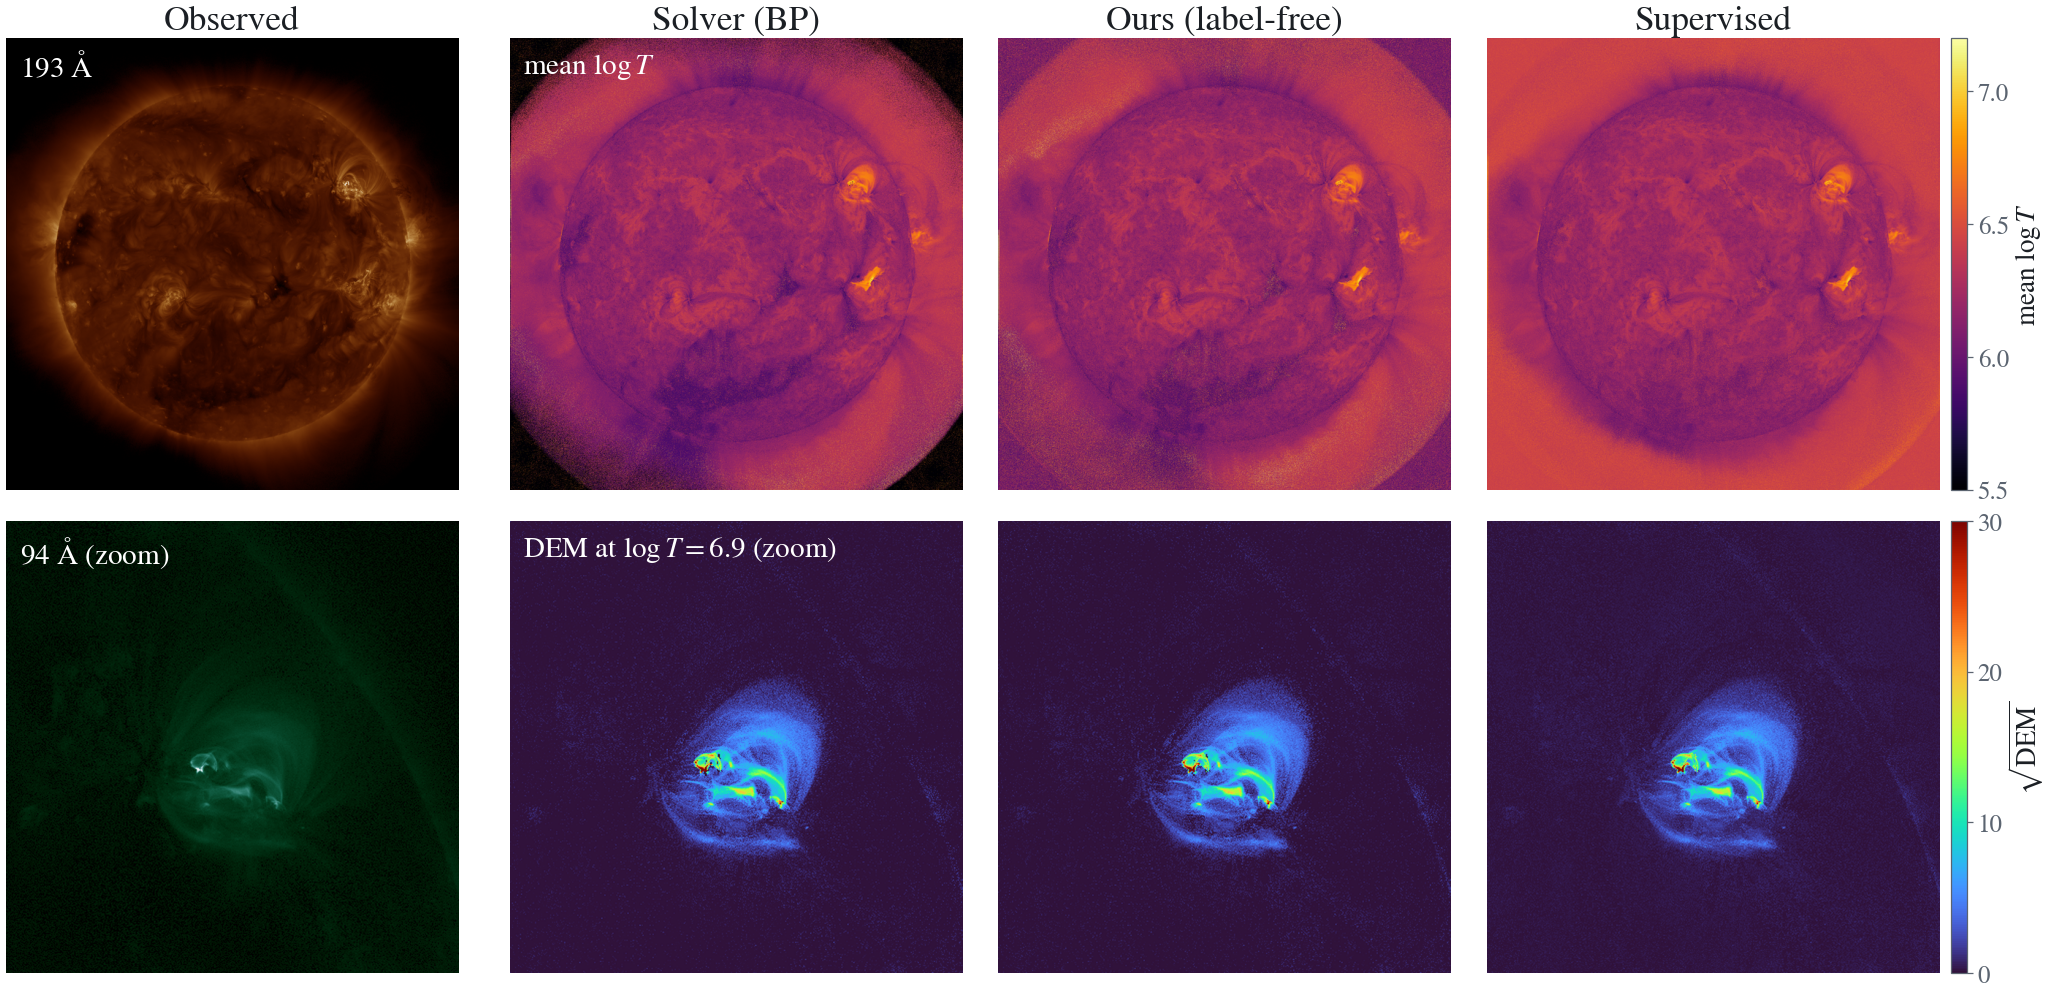
\includegraphics[width=\linewidth]{fig_disk.png}
  \caption{One held-out image from 30 September 2015. Top: the observed 193\Ang{} channel and the mean \logT{} of the DEM from the BP solver, our label-free model and the supervised baseline. Bottom: a zoom on an active region in the observed 94\Ang{} channel, and the DEM in the bin at $\logT=6.9$ (8\,MK). Our model never saw a solver DEM in training. We blank pixels flagged by the self-check of \cref{sec:capacity} in our maps.}
  \label{fig:disk}
\end{figure*}

The corona radiates in the extreme ultraviolet (EUV), and the brightness of each spectral channel depends on how much plasma lies along the line of sight at the temperatures that channel responds to. The differential emission measure (DEM) inverts this relation. For each line of sight it gives the amount of plasma per temperature bin, separating the corona near 1\,MK from flare plasma near 8\,MK, and it is a standard diagnostic of coronal thermal structure. The Atmospheric Imaging Assembly (AIA)~\cite{lemen2012aia} on the Solar Dynamics Observatory~\cite{pesnell2012sdo} images the full Sun at $4096\times4096$ pixels every 12 seconds in seven EUV channels, six of which serve DEM inversion, so in principle one can estimate a DEM for every pixel of every image.

The inversion is both slow and ill-posed. Six intensities cannot determine a DEM on 18 temperature bins, a difficulty known for fifty years~\cite{craig1976limitations}, so every solver adds a regularizer and its answer depends on that choice. We work with two. Basis Pursuit (BP)~\cite{cheung2015dem} finds the smallest total weight on a fixed basis that reproduces every channel within a noise band, which is a linear program (LP). Elastic Net~\cite{athiray2024enet} fits the same basis by regularized least squares. Both solve one problem per pixel. On our $2048\times2048$ grid a BP image is 4.2 million LPs, and one job, including deconvolution and retries, took 9.5 minutes on 16 cores. Inverting 1,223 images with both solvers took 2,446 cluster jobs and produced 1.74\,TB.

Neural emulators move this cost into training. DeepEM~\cite{wright2019deepem} regressed BP's output from AIA intensities, and DEMNet~\cite{perezdiaz2026demnet} extends the idea with Fourier-feature inputs, an uncertainty head and a final stage of forward-model finetuning. Inference becomes one forward pass, but such a model stays bound to its labels. It needs solver output for every training image, a change of solver settings invalidates that output (we discarded 886\,GB of our own Elastic Net labels when the reference regularization weight changed), and the network learns whatever the solver did, including fits to instrument artifacts.

We remove the labels. We train a per-pixel network to minimize the solver's own objective, on about 30 million pixels per epoch. This is amortized optimization~\cite{amos2023tutorial}: instead of searching for each pixel's solution, we learn a function that maps an observation to it. The objective needs only the observations, their noise and the instrument response, so no solver DEM enters training. Solver output appears only through a validity flag, a screen used to choose one loss weight, and the final evaluation, which also informed five model choices. \Cref{fig:disk} shows the result on an image the model never saw.

Removing the labels moves the difficulty into the loss. Elastic Net is already smooth, but BP has a hard constraint, which we replace by a squared penalty with weight $\mu$. Our first BP models used $\mu=1$ and looked excellent on the typical pixel, yet at flare cores they held only 40\% of the solver's emission. Oversampling those pixels, longer training and a 10M-parameter network did not help. The loss was at fault: at $\mu=1$ it charges more to keep the hot plasma than to leave it out (\cref{fig:curves}).

We make three contributions.
\begin{itemize}
\item \textbf{Label-free inversion at full-disk scale.} A per-pixel MLP trained only on the solver's objective. On 153 held-out images, against a supervised baseline scored on the same pixels, it leads on five of six headline measures on Elastic Net and ties the sixth, and it leads on four of six on BP with a median pixel error 3.6 times lower (\cref{sec:comparison}). To our knowledge no earlier DEM network trains without solver labels.
\item \textbf{A calibration of the penalty weight.} Building on a classical result for penalized LPs~\cite{mangasarian2004newton}, we give the distance each channel settles outside its band and the threshold above which that distance is exact, both computable without training a network (\cref{sec:law,sec:verify}). Comparing a network with the per-pixel minimizer of its loss, an amortization gap~\cite{cremer2018inference}, then separates loss failures from training failures. This located our flare-core failure in the loss (\cref{sec:gap,sec:flare}).
\item \textbf{An account of capacity blow-ups.} Wider models failed by orders of magnitude on a few pixels out of 705 million. Most of those pixels were inputs our own training mask had removed, and masking single channels instead of dropping whole pixels removes most of the score blow-ups, though not the most extreme reconstructions. One flare pixel dominated the worst score and is not explained this way (\cref{sec:capacity}).
\end{itemize}

\section{Related work}
\label{sec:related}

\paragraph{DEM inversion.}
Classical approaches include Markov chain Monte Carlo~\cite{kashyap1998mcmc}, regularized inversion~\cite{hannah2012regularized}, fast approximate schemes~\cite{plowman2013fast,plowman2020simple}, sparse inversion by Basis Pursuit~\cite{cheung2015dem,chen1998basis} and Elastic Net~\cite{athiray2024enet,zou2005elastic}. We take the last two as given and ask how to amortize them without running them.

\paragraph{Neural emulators for solar data.}
Szenicer \etal~\cite{szenicer2019virtual} train deep networks on AIA images to predict irradiance, and SuperSynthIA~\cite{wang2024supersynthia} produces full-disk magnetograms from per-pixel distribution outputs. For DEMs, DeepEM~\cite{wright2019deepem} regresses BP's output. DEMNet~\cite{perezdiaz2026demnet} does the same at scale and then finetunes on a forward-model term, and Balodhi and Morton~\cite{bayesdem2026} mix a forward-model term with a loss on regularized-inversion DEMs and estimate uncertainty with dropout. All three need solver DEMs. DEMNet notes that a forward-model term is hard to optimize from scratch because negative solutions also minimize it. We avoid this by predicting the solver's non-negative weights and training on its whole objective, which fixes the tie-break as well as the fit. To our knowledge no earlier DEM network trains without solver labels.

\paragraph{Amortized and constrained optimization.}
Amortized optimization replaces repeated solves with a learned map~\cite{amos2023tutorial}. LISTA~\cite{gregor2010lista} did this for sparse coding by regressing solver output. Closer to us are methods that train on the objective itself. Ablin \etal~\cite{ablin2019unfolded} train unfolded ISTA on the Lasso cost, and other work learns constrained programs without solver labels through completion and correction~\cite{donti2021dc3}, Lagrangian duality~\cite{fioretto2020lagrangian}, primal-dual training~\cite{park2023primal}, feasibility layers~\cite{chen2024e2elr} and exact penalties~\cite{benslimane2025penalty}; Kotary \etal~\cite{kotary2021survey} give a survey. Those methods mostly aim at feasibility on structured problem families. Our instances are tiny but numerous, observation noise makes a small violation harmless, and the question is how large that violation is at a given weight. The relevant theory is the classical penalty method~\cite{courant1943variational,fiacco1968nonlinear,nocedal2006numerical}, usually read as a convergence result. Mangasarian~\cite{mangasarian2004newton} showed that a finite penalty on an LP already recovers an exact dual solution, and we use that fact as a calibration. Physics-informed networks~\cite{raissi2019pinn} use similar weighted penalties and show the same training stiffness as the weight grows~\cite{wang2021pathologies,krishnapriyan2021failure}.

\paragraph{Forward models in vision and astronomy.}
Deep inverse-problem methods~\cite{ongie2020inverse} often fit one scene through a differentiable forward model, from deep image priors~\cite{ulyanov2018dip} to neural fields for black-hole emission~\cite{levis2022bhnerf,feng2026pidef} and the cosmic web~\cite{zhao2025cosmic}. We share the forward-model loss but amortize over pixels and images, so no optimization runs at test time. Our analysis of blow-ups connects to work on how networks behave far from their training data~\cite{hein2019relu,xu2021extrapolate}.

\section{Background}
\label{sec:background}

\paragraph{Forward model.}
At one pixel, AIA gives six intensities $o\in\mathbb{R}^6$ in DN/s, detector counts per second (the 94, 131, 171, 193, 211 and 335\Ang{} channels). A DEM $x\in\mathbb{R}^{18}_{\ge 0}$ on bins from $\logT=5.5$ to $7.2$ produces expected intensities $Rx$, where the response matrix $R\in\mathbb{R}^{6\times 18}$ comes from instrument calibration~\cite{boerner2012calibration}. Both solvers write the DEM as $x=Bw$, with 54 non-negative weights on a fixed basis $B$: at each bin one spike and two Gaussians in \logT{} of width 0.1 and 0.2\,dex (a dex is a factor of ten). With $D=RB$, the predicted intensities are $Dw$. DEM values and weights are in units of $10^{26}\,\mathrm{cm}^{-5}$.

\paragraph{Noise.}
Each reading has a noise estimate $\sigma_c$ from AIA's instrument model~\cite{barnes2020aiapy}. Shot noise dominates at bright pixels, so the relative noise falls with brightness: at the median pixel $\sigma/o$ is about 1.1 in 94\Ang{} and below 0.1 in 171, 193 and 211\Ang. We write $h_c=t\sigma_c$ for the half-width of the noise band of channel $c$, with $t=1.4$ as in BP's first attempt.

\paragraph{Basis Pursuit.}
For each pixel BP solves
\begin{equation}
  \min_{w\ge 0}\ \sum_{k} w_k \quad\text{s.t.}\quad o_c-h_c\le (Dw)_c\le o_c+h_c\ \ \forall c.
  \label{eq:bp}
\end{equation}
Every DEM inside the band is acceptable and the smallest total weight breaks the tie. As a pixel brightens, its band narrows relative to the signal and can become tighter than the accuracy of $R$, a likely reason why some pixels have no feasible DEM. The solver retries those pixels with the band three and then five times wider.

\paragraph{Elastic Net.}
The second solver fits the same weights by
\begin{equation}
  \min_{w\ge 0}\ \frac{1}{2C}\sum_{c}\Bigl(\frac{(Dw)_c-o_c}{h_c}\Bigr)^2
  +\alpha\rho\,\|w\|_1+\frac{\alpha(1-\rho)}{2}\|w\|_2^2,
  \label{eq:enet}
\end{equation}
with $\alpha=0.001$, $\rho=0.5$ and $C=6$ as in the reference run. The $\ell_2$ term spreads weight over more elements, so its DEMs are broader than BP's~\cite{zou2005elastic}.

\paragraph{Why hot plasma is hard to see.}
One unit of plasma at 1 to 1.3\,MK gives 36 to 95\,DN/s in 171\Ang, but one unit at 8\,MK gives no channel more than 0.4\,DN/s. At ordinary pixels the 94\Ang{} signal comes free with warm plasma that the low-noise channels demand anyway. At flare cores most of it comes from hot plasma that only 94 and 131\Ang{} ask for, and a bright reading needs hundreds of units. How a method prices those units decides whether the hot plasma appears in the DEM at all.

\section{Method}
\label{sec:method}

\subsection{Amortized objective}

Let $L(w;o,\sigma)$ be the solver's objective at one pixel. We train one network $f_\theta$ over the pixels of the training set,
\begin{equation}
  \theta^\star=\argmin_\theta\ \sum_{p} L\bigl(f_\theta(o_p);\,o_p,\sigma_p\bigr).
  \label{eq:amortized}
\end{equation}
No solver DEM enters \cref{eq:amortized}. The network sees only the six intensities of one pixel, neither its neighbors nor $\sigma$, which the loss alone uses (\cref{fig:pipeline}).

\begin{figure}[t]
\centering
\begin{tikzpicture}[
  font=\footnotesize,
  box/.style={draw=black!60, rounded corners=1.5pt, minimum height=5.6mm, inner sep=2.5pt, align=center},
  loss/.style={box, fill=black!6},
  arr/.style={-{Stealth[length=4pt]}, black!70, line width=0.4pt}]
  \node[box] (o) {$o$\\[-1pt]{\scriptsize 6 intensities}};
  \node[box, right=4.5mm of o] (f) {$\sqrt{\cdot}$ + Fourier\\[-1pt]{\scriptsize MLP, SiLU}};
  \node[box, right=4.5mm of f] (w) {$w\ge0$\\[-1pt]{\scriptsize 54 weights}};
  \node[box, right=4.5mm of w] (x) {DEM $Bw$\\[-1pt]{\scriptsize 18 bins}};
  \node[box, below=4.5mm of w] (r) {$Dw$\\[-1pt]{\scriptsize predicted intensities}};
  \node[loss, left=6mm of r] (l) {$\sum_k w_k+\mu\sum_c (v_c/h_c)^2$\\[-1pt]{\scriptsize BP loss, no solver output}};
  \draw[arr] (o) -- (f);
  \draw[arr] (f) -- (w);
  \draw[arr] (w) -- (x);
  \draw[arr] (w) -- (r);
  \draw[arr] (r) -- (l);
  \draw[arr] (o.south) -- node[right, inner sep=1.5pt] {\scriptsize $o,\sigma$} (o.south |- l.north);
\end{tikzpicture}
\caption{Training. The network maps one pixel's six intensities to the solver's 54 weights. The loss compares the predicted intensities with the observation and its noise band and adds the total weight.}
\label{fig:pipeline}
\end{figure}

We take the square root of each intensity and lift it to sines and cosines at 12 fixed frequencies~\cite{tancik2020fourier,mildenhall2020nerf}, giving 150 inputs together with the roots themselves. Four hidden layers with SiLU activations~\cite{elfwing2018silu} feed a linear layer and a softplus that keeps the weights non-negative. The final BP model is 680 wide (1.5M parameters) and the Elastic Net model 336 wide (409k). The network outputs the solvers' own variable, the 54 weights, instead of the 18 DEM bins, so it searches the same space as the solver and BP's sparsity term means the same thing for both.

\subsection{Losses}

For Elastic Net, $L$ is \cref{eq:enet} itself. For BP we need a differentiable objective for any output, including outputs outside the band, and the hard constraint becomes a squared hinge:
\begin{equation}
  L_{\mathrm{BP}}(w)=\sum_{k} w_k+\mu\sum_{c}\Bigl(\frac{v_c(w)}{h_c}\Bigr)^2,
  \label{eq:loss-bp}
\end{equation}
where $v_c(w)=\max\bigl(0,\,|(Dw)_c-o_c|-h_c\bigr)$ is the distance outside the band in DN/s. Inside the band the penalty vanishes, so no fit term remains and the sparsity term breaks ties as it does in BP. Dividing by $h_c$ makes one half-width outside cost the same in every channel. Both losses are convex in $w$ for each pixel.

\subsection{What the penalty weight does}
\label{sec:law}

$L_{\mathrm{BP}}$ is the quadratic exterior penalty of the LP~\eqref{eq:bp}~\cite{courant1943variational,fiacco1968nonlinear,nocedal2006numerical}. The textbook result is that its minimizer approaches the LP's solution as $\mu\to\infty$, and Mangasarian~\cite{mangasarian2004newton} showed that a large enough finite weight already gives an exact dual solution. Training needs a more specific statement: where does a pixel settle at a given $\mu$, and when does that answer stop being accurate?

Let $y^\star$ be the LP's dual solution, positive where a lower band edge binds and negative where an upper edge binds, and let $\lambda_c=|y^\star_c|$, the total weight saved per DN/s by which that edge is relaxed. Let $d_c=v_c/h_c$ be the violation in half-widths.

\begin{proposition}
\label{prop:law}
Suppose the LP~\eqref{eq:bp} is feasible with unique primal and dual solutions $w^\star$ and $y^\star$, with support $S$ and binding channels $A$, and let $q=D_{A,S}^{-1}(y^\star_A\circ h_A^2)$. There is a finite $\mu_0$ such that for every $\mu\ge\mu_0$ a minimizer of \cref{eq:loss-bp} is zero off $S$, equals
\begin{equation}
  w_{\mu,S}=w^\star_S-\frac{q}{2\mu}
  \label{eq:path}
\end{equation}
on $S$, and has in every channel
\begin{equation}
  d_c=\frac{\lambda_c h_c}{2\mu}=\frac{\lambda_c\,t\sigma_c}{2\mu}.
  \label{eq:law}
\end{equation}
Moreover $\mu_0$ is the largest $\mu$ at which \cref{eq:path} stops being valid: an element reaches zero, at $\mu=q_k/(2w^\star_k)$, or a free channel reaches a band edge.
\end{proposition}

\Cref{app:proof} gives the proof, but the law itself is a balance of gradients. Stepping $v$ outside the band saves $\lambda v$ in total weight at a constant rate, while the penalty $\mu(v/h)^2$ has slope $2\mu v/h^2$, and the minimizer sits where the two slopes match. A pixel therefore settles further out when light in that channel is expensive, when the reading is noisy, and when $\mu$ is small.

\paragraph{Prices.}
When a single edge binds, the LP buys light from the most efficient basis element, and $\lambda_c=1/\max_k D_{ck}$, the single-edge price of \cref{tab:threshold}. A unit of weight buys at most 0.68\,DN/s of 94\Ang{} but about 290\,DN/s of 171\Ang, so 94\Ang{} is over 400 times more expensive. Real pixels usually bind several edges, and their prices can differ from this value.

\paragraph{From a tolerance to $\mu$.}
Inverting \cref{eq:law}, a tolerance of $\varepsilon$ half-widths needs $\mu\ge\lambda_c h_c/(2\varepsilon)$. With the single-edge price this takes only $R$, $B$ and $\sigma$, with no solver and no training. Take a typical flare core with a 94\Ang{} reading of 164\,DN/s and $\sigma=11.5$, so $h=16.1$ and the band runs from 148 to 180. \Cref{eq:law} gives $d=11.9/\mu$ half-widths, and $\varepsilon=0.1$ needs $\mu\approx120$. Because $\lambda_c$ and $\sigma_c$ vary, no single $\mu$ suits every pixel, so the law does not pick a value but tells us what each value buys. At feasible pixels a larger $\mu$ is always closer to the LP, which leaves training as the upper limit on $\mu$.

\paragraph{Dropping plasma.}
Below $\mu_0$ the law breaks because an element leaves the solution or a free channel reaches an edge, and \cref{eq:path} says when. A one-element model shows how this scales. Take a channel whose signal can only be bought from an element of yield $r=1/\lambda$, with band floor $\ell=o-h$. Minimizing $w+\mu\bigl((\ell-rw)/h\bigr)^2$ over $w\ge 0$ gives
\begin{equation}
  r w^\circ=\max\Bigl(0,\ \ell-\frac{\lambda h^2}{2\mu}\Bigr),
  \label{eq:clip}
\end{equation}
and all of that plasma is dropped once
\begin{equation}
  \mu\le\mudrop=\frac{\lambda h^2}{2\ell}.
  \label{eq:drop}
\end{equation}
For a shot-noise-limited reading, $\sigma^2=g\,o$ with $g$ fixed by the channel and exposure time. Then for $o\gg h$,
\begin{equation}
  \mudrop\approx\frac{\lambda\,t^2 g}{2},
  \label{eq:drop-shot}
\end{equation}
which does not depend on brightness: a brighter pixel needs proportionally more plasma, but the penalty for leaving it out, $(o/h)^2=o/(t^2 g)$, grows at the same rate. At typical noise only 94\Ang{} exceeds 1 (\cref{tab:threshold}), and at the flare core above $\mudrop=1.3$. At $\mu=1$ the first unit of plasma costs 1 and saves only 0.77 of penalty, so the minimum buys none for this channel, whereas at $\mu=100$ it buys until the reading is 0.12 half-widths, about 2\,DN/s, short of the band.

\begin{table}[t]
\centering
\small
\caption{Per-channel single-edge price in weight units per DN/s, noise ratio $g=\sigma^2/o$ (median over bright, high-signal validation pixels), and the resulting threshold \eqref{eq:drop-shot}. Short flare exposures raise $g$ and the threshold in some channels.}
\label{tab:threshold}
\begin{tabular}{@{}lcccccc@{}}
\toprule
Channel (\AA) & 94 & 131 & 171 & 193 & 211 & 335\\
\midrule
Price & 1.48 & 0.10 & 0.0034 & 0.0070 & 0.026 & 0.60\\
$g$ & 0.81 & 0.81 & 0.76 & 0.58 & 0.38 & 0.73\\
\mudrop & \textbf{1.18} & 0.08 & 0.003 & 0.004 & 0.009 & 0.43\\
\bottomrule
\end{tabular}
\end{table}

\paragraph{Infeasible pixels.}
If no $w$ fits every band, the violations cannot vanish and \cref{eq:law} does not apply. A larger $\mu$ then makes the penalty dominate the loss, and the minimizer tends to the closest fit at any weight, whereas the solver returns the smallest weight inside a widened band.

\subsection{Separating loss failures from training failures}
\label{sec:gap}

Because $L_{\mathrm{BP}}$ is convex per pixel, we can find its minimizer $w^\circ(o,\sigma)$ numerically without a network, using L-BFGS-B, and no network can score better on that pixel. This gives two tests. The \emph{amortization gap}~\cite{cremer2018inference} compares the network's loss with that of $w^\circ$: if the gap is small and the result is poor, the loss itself is at fault and more training cannot help. The \emph{screen} scores $w^\circ$ against the solver's DEM for each candidate $\mu$, evaluating a loss on held-out pixels without training a model.

\subsection{Clamped channels}
\label{sec:clamp}

PSF deconvolution can produce negative intensities, and these are then set to zero. We call a channel clamped when it reads at most $10^{-3}$\,DN/s, and 40\% of valid pixels in our data have such a channel, nearly all of them faint. A clamped reading is an artifact, so a band around it asks for the wrong thing. Dropping the whole pixel, as we first did, removes every input containing a zero from the training set. \emph{Channel masking} instead keeps the pixel and removes only that channel's penalty: the other channels keep their bands, and the network still reads the zero as an input.

\subsection{Training}

Each epoch draws 512 fresh pixels from each of 58,688 blocks of $128\times128$ pixels, about 30M pixels, in batches of 16 blocks. We use Adam~\cite{kingma2015adam} at a peak learning rate of $3\times10^{-4}$ with no weight decay, a linear warm-up (500 steps for BP, 3,000 for Elastic Net), cosine decay and gradient-norm clipping at 1. The final BP model trains for 120 epochs with $\mu=100$ and channel masking, in 6.6 hours on one GPU. The Elastic Net model trains for 40 epochs without clamped pixels. \Cref{app:engineering} describes a silent collapse at the start of training and a sampling bug, with their fixes.

\section{Data and evaluation protocol}
\label{sec:protocol}

\paragraph{Data.}
We use 1,223 full-disk AIA images from 2014 and 2015, about two per day. We deconvolve them with revised point-spread functions~\cite{hofmeister2025psf} and correct for exposure time and degradation. DEMs live on a $2048\times2048$ grid, with DEM pixel $(i,j)$ reading AIA pixel $(2i,2j)$. We cut each image's grid into 256 blocks and keep a random 64. The split is in time: 917 images for training (to 16 June 2015), 153 for validation and 153 for test (21 September to 31 December 2015, on 86 distinct days).

\paragraph{Shared test set.}
We use the evaluation protocol and scripts of DEMNet's authors and score both models on the same pixels against the same solver DEMs. Each test image has five targets, the solve of the clean image and four re-solves with Gaussian noise of $0.5\sigma$ added, and the input is the clean image for all five. The protocol scores each target on a random 64 of the image's 256 blocks, giving 48,960 blocks and 802M pixel-targets on Elastic Net. On BP 705M of these carry a solver DEM. The missing share at clean solves, 7.7\%, is close to the 8.5\% of pixels our own solver run had to relax, so the missing targets appear to be the infeasible pixels, and BP scores then describe feasible pixels only.

\paragraph{Brightness.}
A pixel is Bright when any channel reaches that channel's top-5\% cutoff and Quiet otherwise. Flare cores are pixels with some channel at 32 times its cutoff or more, which in 94\Ang{} means 100\,DN/s: 69,283 of the 705M, about one pixel in 10,000. They are the brightest pixels of flaring active regions rather than flare peaks alone. The strongest flare in the test window is close to X1, on 28 September 2015.

\paragraph{Measures.}
DEM MAE and MSE average over pixels and the 18 bins. EM error is the summed absolute error in total emission over the summed solver emission. W1 is the Wasserstein distance in dex between the two DEMs normalized as distributions over \logT. AIA MAE and MSE compare each DEM's predicted intensities with the observation in DN/s. These six are the headline measures. The per-pixel error is the squared error summed over the bins, and we report its percentiles because it is heavy-tailed: on an early model, one pixel in five million held 94\% of the mean training loss and reversed a model ranking. Flare-core emission and 94\Ang{} reproduced are ratios of sums over flare cores.

\paragraph{Baseline.}
The supervised baseline uses the DEMNet architecture~\cite{perezdiaz2026demnet}: 1.05M parameters, regression and classification heads over the DEM bins, and 140 epochs on solver DEMs from the same deconvolved images, with a resynthesis term of weight 0.01 from epoch 100. We use one checkpoint per solver from DEMNet's authors and evaluate both ourselves, on the same pixels and with the same code as our models. On BP the checkpoint scores DEM MSE 0.91 and AIA MSE 157.

\paragraph{Model selection.}
We chose widths, inputs and checkpoints on the training loss, which needs no solver DEM. During training we logged it on 131,072 pixels from the first four validation images, a sample too small for the rarest pixels that, with clamped pixels dropped, contains none of the inputs that fail. We therefore also scored the candidates on every pixel of the 153 validation images (\cref{sec:allpixels}), and that pass supports the final BP model. The Elastic Net width, epochs and treatment of clamped pixels rest on test scores, as does the rejection of the widened band in \cref{sec:infeasible}. The penalty weight came from a screen against solver DEMs on validation. \Cref{app:selection} gives the details.

\section{Results}
\label{sec:results}

\subsection{Comparison with a supervised baseline}
\label{sec:comparison}

\begin{table}[t]
\centering
\small
\caption{Shared test set, same pixels and targets for both models. Bold marks the better of a pair when the two differ by 3\% or more; we have no seed spread, so smaller differences count as ties, as do pairs of percentiles one histogram bin (0.02\,dex) apart. Lower is better except in the last two rows, where the target is the solver's own value: 100\% for emission and, for 94\Ang, 92\% on BP and 55\% on Elastic Net.}
\label{tab:headline}
\begin{tabular}{@{}lcccc@{}}
\toprule
 & \multicolumn{2}{c}{Basis Pursuit} & \multicolumn{2}{c}{Elastic Net}\\
\cmidrule(lr){2-3}\cmidrule(l){4-5}
Measure & Ours & Sup. & Ours & Sup.\\
\midrule
DEM MAE & \textbf{0.072} & 0.100 & \textbf{0.151} & 0.188\\
DEM MSE & 1.08 & \textbf{0.91} & 0.310 & 0.318\\
EM error (\%) & \textbf{11.0} & 14.3 & \textbf{12.2} & 18.0\\
W1 (dex) & \textbf{0.070} & 0.133 & \textbf{0.103} & 0.121\\
AIA MAE (DN/s) & 3.54 & \textbf{2.95} & \textbf{0.56} & 6.32\\
AIA MSE & \textbf{148} & 157 & \textbf{161} & 598\\
\midrule
Median pixel error & \textbf{0.031} & 0.112 & \textbf{0.85} & 1.12\\
p90 & 1.86 & 1.95 & \textbf{7.76} & 8.51\\
p99 & 25.7 & 26.9 & \textbf{29.5} & 35.5\\
p99.9 & 170 & 162 & \textbf{102} & 178\\
\midrule
Quiet MSE & 0.0331 & 0.0335 & \textbf{0.122} & 0.130\\
MSE without flare cores & \textbf{0.087} & 0.091 & \textbf{0.172} & 0.210\\
Flare-core emission (\%) & \textbf{96.7} & 92 & \textbf{99} & 87\\
Flare-core 94\Ang{} (\%) & 88 & 85 & \textbf{53} & 48\\
\bottomrule
\end{tabular}
\end{table}

\Cref{tab:headline} compares our final models with the supervised baseline. On Elastic Net our model leads on five of the six headline measures and ties on DEM MSE (0.310 against 0.318). Its AIA MAE is eleven times lower than the baseline's and also lower than the solver's own 1.41\,DN/s, though the solver's AIA MSE (134) is lower than ours. That tie depends on a test-informed choice: at 120 epochs, which the validation loss preferred, our DEM MSE is 0.362 and the baseline would lead.

On BP our model leads on four of the six, and the baseline keeps DEM MSE (0.91 against 1.08) and AIA MAE (2.95 against 3.54). BP's own AIA MAE on these pixels is 4.26\,DN/s, worse than either network, because the solver only has to land inside the band, while its AIA MSE (61.9) beats both. The BP mean and median disagree because the error is heavy-tailed. On the typical pixel our model is 3.6 times closer to the solver (0.031 against 0.112), and from the 90th percentile upward the two are level within the resolution of our histograms. Flare cores, one pixel in 10,000, hold 92.0\% of our squared error and 90.0\% of the baseline's. Without them our DEM MSE is slightly lower (0.087 against 0.091), so the BP DEM MSE gap comes from flare cores, where our error is 1.22 times the baseline's.

The clearest differences between the two models are in shape, which the means hide. At BP flare cores the baseline falls 10\% to 22\% short of the observed 131 to 211\Ang, while ours stays within 1\% (\cref{tab:channels}). The baseline flags 41.1\% of pixels as multi-peaked at 24\% precision against the solver, and ours flags 12.8\% at about 63\%, with the solver itself at 13.5\%. W1, which measures where emission sits in temperature, is about half the baseline's.

The five targets also bound what any deterministic model can do. Where several targets cover a block, the MSE splits into the distance to the mean solver DEM and the solver's own scatter across re-solves. For our BP model that scatter is 43.9\% of the Quiet error and 0.3\% of the flare-core error. Nearly half of the remaining Quiet error is the solver disagreeing with itself under half-$\sigma$ noise, while the flare-core error belongs to the model.

\subsection{The flare-core failure was in the loss}
\label{sec:flare}

\begin{figure}[t]
  \centering
  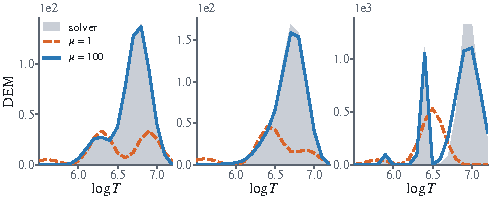
\includegraphics[width=\linewidth]{fig_curves.pdf}
  \caption{Three random flare cores from validation, among those with a solved LP and a binding 94\Ang{} lower edge: the solver's DEM against the numerical minimizer of the loss. At $\mu=1$ the hot peak disappears. No network is involved.}
  \label{fig:curves}
\end{figure}

\begin{table*}[t]
\centering
\small
\caption{BP runs on the shared test set. Flare-core columns are percentages (solver: 100 and 92). The bold row is the final model, the only one with channel masking; every other label-free row drops clamped pixels. The 360k model uses a logarithmic input and all others the square-root Fourier input.}
\label{tab:runs}
\setlength{\tabcolsep}{4.5pt}
\begin{tabular}{@{}llccccccc@{}}
\toprule
Loss & Model & Epochs & DEM MSE & Median & AIA MSE & Quiet MSE & Emission & 94\Ang\\
\midrule
$\mu=1$ & 360k & 40 & 4.28 & 0.026 & 83 & 0.058 & 40 & 23\\
 & 409k & 40 & 4.56 & 0.023 & 83 & 0.057 & 35 & 15\\
 & 409k, flare cores oversampled & 40 & 5.05 & 0.025 & 87 & 0.058 & 24 & 9\\
 & 409k & 120 & 4.21 & 0.022 & 108 & 0.057 & 37 & 16\\
 & 10M & 40 & 5.10 & 0.022 & 125 & 0.058 & 20 & 8\\
\midrule
$\mu=100$ & 409k & 40 & 2.37 & 0.062 & 44 & 0.035 & 89 & 68\\
 & 409k & 120 & 2.00 & 0.041 & 44 & 0.032 & 92 & 75\\
 & 409k & 120+120 & 1.75 & 0.036 & 103 & 0.032 & 93 & 77\\
 & 1.5M & 120 & 897 & 0.034 & 21.7M & 12.5 & 115 & 78\\
 & \textbf{1.5M, channels masked} & \textbf{120} & \textbf{1.08} & \textbf{0.031} & \textbf{148} & \textbf{0.033} & \textbf{97} & \textbf{88}\\
\midrule
$\mu=300$, solver's band & 409k & 120 & 1.54 & 0.045 & 116 & 0.050 & 97 & 87\\
\midrule
\multicolumn{2}{@{}l}{Supervised baseline} & & 0.91 & 0.112 & 157 & 0.033 & 92 & 85\\
\bottomrule
\end{tabular}
\end{table*}

At $\mu=1$ our first production model reproduced 171, 193 and 211\Ang{} at flare cores to within 2\%, but only 23\% of 94\Ang, 76\% of 131\Ang{} and 67\% of 335\Ang, the channels that see hot plasma, and it held 40\% of the solver's emission. The natural reading is underfitting. \Cref{tab:runs} shows the three obvious remedies on the original loss. Oversampling raised flare cores 8.4-fold in training and made them worse, tripling the epochs moved flare-core emission from 35\% to 37\%, and a 10M-parameter model reached 20\%.

\begin{table}[t]
\centering
\small
\caption{Four answers scored under the original loss ($\mu=1$) at validation flare cores: total loss, its sparsity and penalty terms, the share of observed 94\Ang{} reproduced, and emission relative to the solver.}
\label{tab:gap}
\begin{tabular}{@{}lcccc@{}}
\toprule
Answer & Loss & Sparsity + penalty & 94\Ang & EM\\
\midrule
Network, $\mu=1$ & 565 & 294 + 270 & 28\% & 38\%\\
Minimizer $w^\circ$ & 463 & 220 + 243 & 26\% & 30\%\\
Solver's DEM & 1,125 & 1,119 + 6 & 94\% & 100\%\\
Supervised DEM & 1,878 & 1,107 + 771 & 91\% & 95\%\\
\bottomrule
\end{tabular}
\end{table}

\Cref{tab:gap} gives the diagnosis. The amortization gap was small: the network's median loss sits 8.0\% above the per-pixel minimum at flare cores and 0.8\% to 3.6\% above it from 0.03 to 32 times the Bright cutoff, so training had converged. The minimizer itself reproduces only 26\% of 94\Ang. The loss rates the solver's DEM 2.4 times worse than an answer without the hot plasma, so better training on this loss cannot recover it. \Cref{fig:curves} shows the effect at three random flare cores. The original weight was outside the law's range: $\mu_0$ exceeds 1 at 99.9\% of solved flare cores. Extrapolating the first linear piece of \cref{eq:path}, a hot element ($\logT\ge6.6$) reaches zero above $\mu=1$ at 96\% of them, with a median of 10.6.

Raising $\mu$ to 100 restores the hot plasma at feasible pixels. With only that change, DEM MSE halves and flare-core emission rises from 35\% to 89\%. Training then becomes the limit: at flare cores the amortization gap is 118\% after 40 epochs and 47\% after 120. Longer training and greater capacity close most of the rest (\cref{tab:runs}). The final model holds 96.7\% of the solver's emission at flare cores and reproduces 88\% of 94\Ang, against 92\% for the solver and 85\% for the baseline.

The same mechanism explains a milder effect at ordinary pixels. Nothing pulls a channel toward its observation inside the band, so the sparsity term drags emission to the band's lower edge, and a finite $\mu$ lets it slip past. At 0.3 to 1 times the Bright cutoff the minimizer emits 0.861 of the solver's emission at $\mu=1$ and 1.009 at $\mu=100$. Over the test set, emission relative to the solver rose from 0.848 for our first model to 0.988 for the final one.

\subsection{Testing the penalty law}
\label{sec:verify}

\begin{figure*}[t]
  \centering
  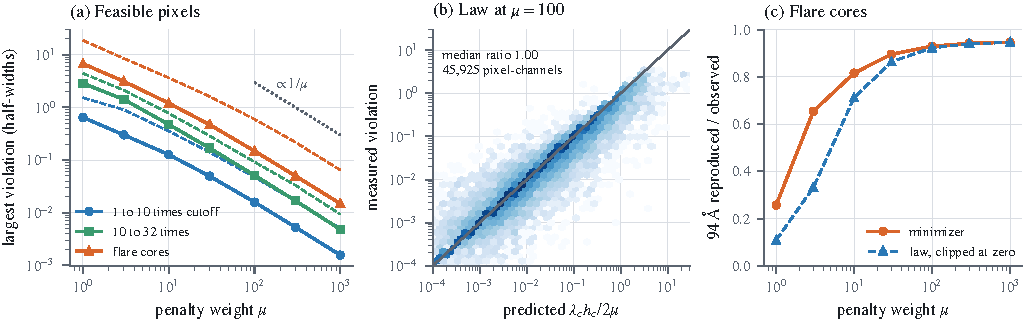
\includegraphics[width=\linewidth]{fig_law.pdf}
  \caption{The penalty law on validation pixels. (a) Largest violation per pixel against $\mu$ at pixels with a solved LP: median (solid) and 90th percentile (dashed), by brightness relative to the Bright cutoff. (b) Measured against predicted violation at $\mu=100$ for every pixel-channel above $10^{-4}$ half-widths. (c) 94\Ang{} reproduced at 4,863 solved flare cores where the 94\Ang{} lower edge binds: the loss's numerical minimizer against \cref{eq:law} using each pixel's LP price, clipped as in \cref{eq:clip}.}
  \label{fig:law}
\end{figure*}

\begin{table}[t]
\centering
\small
\caption{The law by brightness band (multiples of the Bright cutoff) on validation pixels: pixels sampled, share with a solved LP, the median threshold $\mu_0$ of \cref{prop:law}, the share with $\mu_0\le100$, and the $\mu$ that holds the median and the 90th-percentile pixel within 0.1 half-widths.}
\label{tab:law}
\begin{tabular}{@{}lrcccrr@{}}
\toprule
Band & Pixels & Solved & $\mu_0$ & $\le100$ & \multicolumn{2}{c}{$\mu$ for 0.1}\\
\midrule
$<0.03$ & 50 & 100\% & 0.06 & 100\% & 0.2 & 0.4\\
0.03--0.1 & 296 & 99\% & 0.11 & 100\% & 0.3 & 1.4\\
0.1--0.3 & 608 & 99\% & 0.20 & 99\% & 0.6 & 2.5\\
0.3--1 & 1,000 & 94\% & 1.5 & 92\% & 2.3 & 21\\
1--1.8 & 1,000 & 88\% & 8.1 & 87\% & 11 & 44\\
1.8--3.2 & 1,000 & 90\% & 7.6 & 87\% & 13 & 48\\
3.2--10 & 1,000 & 96\% & 10 & 84\% & 25 & 68\\
10--32 & 1,000 & 100\% & 15 & 87\% & 53 & 102\\
$\ge 32$ & 6,000 & 88\% & 37 & 72\% & 168 & 763\\
\midrule
All & 11,954 & 91\% & 18 & 81\% & 64 & 367\\
\bottomrule
\end{tabular}
\end{table}

We solved the LP and the loss at seven values of $\mu$ from 1 to 1,000 on 11,954 validation pixels, 6,000 of them flare cores. The LP has a solution at 10,899 of them, and all but 29 of those are nondegenerate (\cref{tab:law}).

\Cref{prop:law} makes a sharp prediction, because $\mu_0$ can be computed for each pixel from the LP before any penalized solve. Above $1.05\,\mu_0$ the law should hold, and well below it should not. That is what we find. At $\mu=1$, 99.4\% of pixel-channels above their threshold are within 5\% of the prediction, against 3.7\% of those below $0.5\,\mu_0$. The median ratio above the threshold is 1.00 at every $\mu$, and below it 0.49 to 0.70. The share within 5\% falls to 85\% at $\mu=100$ and 68\% at $\mu=1{,}000$, but these misses are optimizer error: at all of the 1,299 and 3,036 pixels involved, \cref{eq:path} has a loss no higher than the L-BFGS-B answer. Over the 45,925 pixel-channels violated at $\mu=100$ the median ratio is 1.00 (\cref{fig:law}b).

\Cref{tab:law} shows that the threshold is low enough to matter in practice. The median $\mu_0$ is below 2 up to the Bright cutoff and 37 at flare cores, and 72\% of solved flare cores have $\mu_0\le100$. Median violations at flare cores fall with a slope of $-0.7$ at small $\mu$ and reach $-1$ from about $\mu=30$ (\cref{fig:law}a). Using LP prices alone, the law reproduces the 94\Ang{} column of the screen from $\mu=30$ upward (0.923 predicted, 0.930 measured at $\mu=100$). At small $\mu$ it underestimates that column (0.11 against 0.26 at $\mu=1$), as expected once the solution has changed support (\cref{fig:law}c). The one-element threshold \eqref{eq:drop} is therefore a guide to scaling rather than a pixel-level predictor. Its median at flare cores is 1.32, against 37 for the exact $\mu_0$.

The prices match \cref{sec:law}. At flare cores the median 94\Ang{} price is 1.46, close to the single-edge value of 1.48, although every solved flare core binds three to six edges. It exceeds that value at 49\% of them (99th percentile 8.8). 94\Ang{} has the largest predicted violation at 70\% of flare cores, 335\Ang{} at 15\% and 131\Ang{} at 13\%. With measured prices $\mudrop$ exceeds 1 for 131\Ang{} at 17\% of solved flare cores, and for 193 and 335\Ang{} at 3\%. The noise ratio behaves as \cref{eq:drop-shot} assumes: in 94\Ang{} at flare cores $g$ runs from 0.806 to 0.817 between the 10th and 90th percentiles.

The screen in \cref{tab:screen} kept $\mu=100$ before we had the law, and the law says what that choice means. At $\mu=100$ the median solved flare core sits 0.15 half-widths outside its band and the 90th percentile 0.60 (predicted 0.17 and 0.76). The value of 120 that \cref{sec:law} obtains from $R$ and the noise alone is close to where the screen's 94\Ang{} column levels off. A single $\mu$ cannot hold every pixel to one tolerance: the hardest solved pixel in the sample, a flare core priced on 335\Ang, would need 63,801 for 0.1 half-widths.

The law describes the minimizer rather than the network, and a network adds its amortization gap on top. At validation flare cores the 409k model at $\mu=100$ (120+120 epochs) has a median worst-channel violation of 0.79 half-widths against the minimizer's 0.18, with a maximum of 1,695. We have not made this measurement on the final model.

\subsection{Pixels where no DEM fits the band}
\label{sec:infeasible}

\begin{table}[t]
\centering
\small
\caption{The screen on validation: the loss's minimizer, with no network, scored against the solver. DEM error is the DEM MSE with brightness bands weighted by population. ``Fixed'' keeps the $1.4\sigma$ band everywhere and ``Solver'' widens it where the solver did. Supervised reference: DEM error 6.10, Quiet MSE 0.054.}
\label{tab:screen}
\setlength{\tabcolsep}{4.5pt}
\begin{tabular}{@{}rcccccc@{}}
\toprule
 & \multicolumn{2}{c}{DEM error} & \multicolumn{2}{c}{Quiet MSE} & \multicolumn{2}{c}{Flare core, fixed}\\
\cmidrule(lr){2-3}\cmidrule(lr){4-5}\cmidrule(l){6-7}
$\mu$ & Fixed & Solver & Fixed & Solver & 94\Ang & EM\\
\midrule
1 & 36.9 & 37.8 & 0.076 & 0.074 & 26\% & 30\%\\
10 & 10.9 & 12.1 & 0.037 & 0.027 & 81\% & 90\%\\
30 & 4.94 & 5.47 & 0.034 & 0.015 & 89\% & 97\%\\
100 & 2.30 & 2.79 & 0.046 & 0.0079 & 93\% & 100\%\\
300 & 1.78 & 1.11 & 0.053 & 0.0036 & 94\% & 101\%\\
1000 & 2.17 & 0.63 & 0.055 & 0.0018 & 95\% & 101\%\\
\bottomrule
\end{tabular}
\end{table}

The fixed-band columns of \cref{tab:screen} show a trade-off. Raising $\mu$ first helps and then hurts, and faint-pixel error climbs from $\mu=30$ upward. The cause is one group of pixels. At 8.8\% of the sample, and 12\% of flare cores, the LP has no solution at the $1.4\sigma$ band: 7.8\% are provably infeasible and the rest are numerical failures of the LP solver. These are the pixels the reference solver relaxes. There the violation has a floor set by the observation, and raising $\mu$ pushes the minimizer away from the solver. At 0.3 to 1 times the Bright cutoff its DEM error at those pixels grows from 0.055 at $\mu=1$ to 0.92 at $\mu=100$ and 1.29 at $\mu=1{,}000$. At $\mu=100$ they hold 70\% to 90\% of the minimizer's error between 0.3 and 10 times the cutoff.

Widening the band where the solver widened it, while still measuring the excess in units of the original half-width, removes the trade-off. Every column in \cref{tab:screen} then improves monotonically with $\mu$, and a perfect network would simply want the largest $\mu$.

A real network does not get there. We trained the 409k model for 120 epochs at $\mu=300$ on the solver's band (\cref{tab:runs}). At the targeted pixels it did what the screen predicts, with validation DEM MAE of 0.15 against 0.45 for the same recipe at $\mu=100$, and it improved test DEM MSE and flare-core 94\Ang{} (1.54 and 87\%, against 2.00 and 75\%). But test Quiet MSE rose to 0.050, far above the 0.0036 the minimizer reaches on validation, and one validation pass spiked to $4\times10^{16}$. The loss had improved and the optimization had become harder, a pattern familiar from stiff penalties in physics-informed networks~\cite{wang2021pathologies,krishnapriyan2021failure}. Widening also needs the solver's per-pixel flag, or an LP feasibility check per pixel, which gives back part of what label-free training saves. We therefore keep the fixed band at $\mu=100$, and the final model reaches the same flare-core quality that way. A 1.5M model on the widened band remains untested. Because the BP test targets are missing at these pixels, the headline scores can show neither the gain from widening nor the cost of not widening.

\subsection{Capacity and out-of-distribution inputs}
\label{sec:capacity}

With clamped pixels dropped from training, wider models improved the typical pixel and failed by orders of magnitude on a few others. On Elastic Net with a logarithmic input, models of 722k and 1.43M parameters reached DEM MSE 3.24 and 36.2 against 0.48 at 360k, and with our final input a 10M model reached 2,062 against 0.310 at 409k. The validation loss preferred or tied each of them. On BP at $\mu=100$ a 1.5M model has a median pixel error of 0.034 and a DEM MSE of 897, with 99.7\% of its squared error in its worst 100 of 705M pixels.

Most of these failures share a cause. In those Elastic Net models and the 10M BP model, 93\% to 99\% of the squared error sits in pixels with a clamped channel. The failing inputs are strange. In the 1.5M model's worst 100 distinct inputs a median of five of six channels read at most $10^{-3}$\,DN/s, and in 56\% a single channel has signal, always 94\Ang, at a median 3.0\,DN/s and 28 times the median of its eight neighbors. Such a lone reading looks like a residual cosmic-ray hit or a hot pixel. Our training mask had removed every pixel with a clamped channel, 40\% of pixels rather than the 5\% we first estimated from two channels, and the validation loss used the same mask, so neither had ever contained such an input. In standardized log intensity these inputs sit about 4.9 from the nearest of 2M training pixels, while test pixels above 0.3 times the cutoff sit 0.08 to 0.21 away. Near the data the loss pins the output, and far from it nothing does~\cite{hein2019relu,xu2021extrapolate}. A larger network has more room to bend there: over the 10M Elastic Net model's worst 1,000 inputs the median emission is $1.6\times10^5$ times the solver's. Distance alone does not mark failure, though, since faint pixels can sit as far out without any error.

Channel masking (\cref{sec:clamp}) tests this account. It takes the 10M Elastic Net model from DEM MSE 2,062 to 1.82, though that model keeps an AIA MSE of 148,403, and it brings the 1.5M BP model's Quiet MSE from 12.5 down to 0.033. Smaller models get worse with the same change (BP 409k at 40 epochs from 2.37 to 2.79, Elastic Net 409k from 0.310 to 0.439), possibly because clamped pixels take a large share of each epoch's draws. Our Elastic Net model therefore stays at 409k with clamped pixels dropped.

The 1.5M BP model's DEM MSE needs a separate explanation. It fell from 897 to 1.08, but clamped pixels held only 2.9\% of the 897. One unclamped flare-core input, seen through two targets, held 96.7\%, with 131\Ang{} above 90,000\,DN/s. Masking does not touch that pixel. With one run of each configuration we cannot say why the masked model does not fail on it, so this part of the improvement may be chance and needs repeating with more seeds.

Masking did not remove the most extreme outliers. On eight full disks, 124 of 33.5M pixels are reconstructed above $10^3$\,DN/s and more than 100 times their observation. Of these, 123 have no solver DEM, because they are unsolved even at the widest band, so they enter neither training nor any score. They are mostly single-channel readings among zeros, and simple input rules isolate them poorly: no dominant-channel rule we tried catches more than 79\% of them. A direct self-check works and needs neither a solver nor a label. A DEM must reproduce what was observed, so a pixel reconstructed above $10^3$\,DN/s and more than 100 times its observation is flagged. The paper's scores do not apply this check. The one flagged pixel with a solver DEM holds 97.7\% of our error on its disk.

Spatial context did not help. A patch CNN on a $9\times9$ neighborhood (1.48M parameters), matched in size to a 680-wide MLP and trained on the same data at $\mu=1$, lost to the MLP at every percentile of the training loss on test pixels (BP median 1.01 against 0.98, Elastic Net 0.033 against 0.020). \Cref{app:architecture} gives this comparison and a width sweep.

\section{Discussion and limitations}
\label{sec:discussion}

\paragraph{What the scores mean.}
Every score here is a distance to a regularized solution of an underdetermined problem. No ground-truth DEM exists for these images, so neither our results nor the baseline's show that a DEM is physically right. A label-free model inherits the solver's regularizer through its objective. It emulates the solver's choice of answer and makes no independent claim about the Sun.

\paragraph{Coverage.}
The test window has no flare far above X1, and we did not treat saturated pixels specially, so behavior on large X-class events is untested. Training reads one solver output, the flag that drops the 0.01\% to 0.02\% of pixels the solver could not solve at all. We trained the two 1.5M configurations with three seeds each and the others once. We treat AIA alone, without Hinode/XRT. Our output is a single DEM, whereas DEMNet also predicts a distribution per bin, which we do not attempt.

\paragraph{The remaining gap.}
Our remaining flare-core error is in the height of the tallest peaks. Above a solver peak of 3,200 units our model reaches 0.53 of the solver's peak and the baseline 0.70, and those 269 pixel-targets hold 83\% of our squared error. Part of this is training: at validation flare cores the final model's median amortization gap is 21\%, against 5\% to 12\% elsewhere, and it reproduces 87\% of 94\Ang{} where the minimizer reaches 93\%.

\paragraph{Speed.}
On one NVIDIA B200 GPU the 1.5M and 409k networks take 0.32 and 0.11 seconds per $2048\times2048$ image, or 13.3M and 36.7M pixels per second. On the 16 cores of a solver job they take 36 and 19 seconds. BP took 221 seconds of solving on those cores before any retries, which makes the GPU about 700 times faster for the 1.5M model and the same CPU cores 6 and 12 times faster. Both pipelines still pay about 4 minutes of CPU deconvolution per image, so the end-to-end gain over a 9.5-minute BP job stays near a factor of two until that step also moves to a GPU.

\paragraph{Directions.}
\Cref{prop:law} suggests two refinements, neither trained yet. A per-pixel, per-channel weight proportional to $\lambda_c h_c$, with the single-edge price standing in for $\lambda_c$, needs only $R$, $B$ and $\sigma$ and would hold pixels to a roughly common tolerance. An $\ell_1$ exterior penalty is exact~\cite{han1979exact}: once $\mu$ exceeds $\lambda_c h_c$ in every binding channel (about 24 at the flare core of \cref{sec:law}), its minimizer solves the LP itself, at the cost of a slope that jumps at the band edge.

\section{Conclusion}
\label{sec:conclusion}

Training on a solver's objective is enough to emulate it at full-disk scale. Our per-pixel models never see a solver DEM and hold their own against a supervised baseline scored on the same pixels, although that baseline keeps DEM MSE and AIA MAE on BP and our means remain sensitive to a few pixels. The difficult part was the loss. A hard noise band turned into a penalty behaves as a price, and the LP says what that price is: \cref{eq:law} gives how far outside its band each channel settles, and \cref{prop:law} gives the weight below which that stops being true. At still lower weights hot plasma is lost, which explains a failure that training could not fix. More generally, when a network is trained on an objective rather than on labels, that objective can be solved directly on a sample of inputs, which is a cheap way to learn whether a failure lies in the loss or in the training. We recommend doing this before scaling up.

{
    \small
    \bibliographystyle{ieeenat_fullname}
    \bibliography{refs}
}
\clearpage
\appendix
\renewcommand{\thesection}{\Alph{section}}

\section{Proof of \cref{prop:law}}
\label{app:proof}

Write the LP~\eqref{eq:bp} with edges $\ell_c=o_c-h_c$ and $u_c=o_c+h_c$. Its dual variable $y\in\mathbb{R}^6$ is positive when a lower edge binds and negative when an upper edge binds, and dual feasibility reads $1-\sum_c y_c D_{ck}\ge 0$ for every $k$, with equality on the support of the primal solution.

Let $b_c$ be the binding edge of channel $c\in A$. A unique primal solution makes the columns of $D_{A,S}$ independent and a unique dual solution makes its rows independent, so $D_{A,S}$ is square and invertible. Strict complementarity, which also follows from uniqueness, gives $1-\sum_c y^\star_c D_{ck}>0$ for $k\notin S$. Set $q=D_{A,S}^{-1}(y^\star_A\circ h_A^2)$, $w_{\mu,S}=w^\star_S-q/(2\mu)$ and $w_{\mu,k}=0$ for $k\notin S$. Then
\begin{equation}
  D_{A,S}\,w_{\mu,S}=b_A-\frac{y^\star_A\circ h_A^2}{2\mu},
\end{equation}
so each channel in $A$ sits outside its binding edge by $v_c=\lambda_c h_c^2/(2\mu)$. As $\mu\to\infty$, $w_{\mu,S}\to w^\star_S>0$, and the channels outside $A$, strictly inside their bands at $w^\star$, stay inside. There is therefore a finite $\mu_0$ beyond which $w_{\mu,S}>0$ and $v_c(w_\mu)=0$ for $c\notin A$. It is the largest of $q_k/(2w^\star_k)$ over $k\in S$ with $q_k>0$, and of $D_{c,S}\,q/\bigl(2((Dw^\star)_c-\ell_c)\bigr)$ or $-D_{c,S}\,q/\bigl(2(u_c-(Dw^\star)_c)\bigr)$ over $c\notin A$, according to the sign of $D_{c,S}\,q$.

For $\mu\ge\mu_0$ the gradient of \cref{eq:loss-bp} at $w_\mu$ in coordinate $k$ is
\begin{equation}
  1-\sum_{c\in A}\operatorname{sign}(y^\star_c)\,\frac{2\mu\,v_c}{h_c^2}\,D_{ck}
  =1-\sum_{c}y^\star_c D_{ck},
\end{equation}
which is zero on $S$ and positive off it. These are the optimality conditions of the convex problem $\min_{w\ge0}L_{\mathrm{BP}}$, so $w_\mu$ is a minimizer. Dividing $v_c$ by $h_c$ gives \cref{eq:law}.\hfill$\square$

\paragraph{Remark.}
The same computation shows that at any minimizer of \cref{eq:loss-bp}, for any $\mu$, the vector with entries $\pm 2\mu v_c/h_c^2$ is dual feasible for the LP. Violations are scaled dual variables, which is the content of the exact-penalty result of Mangasarian~\cite{mangasarian2004newton}. That work needs weaker assumptions and recovers the least-norm dual solution. We assume uniqueness because it gives the explicit path \eqref{eq:path} and threshold $\mu_0$, and in our sample all but 29 of 10,899 LP solutions pass the check $|S|=|A|$.

\section{Basis, response and noise}
\label{app:basis}

The basis has a spike and two Gaussians $\exp(-\Delta\logT^2/a^2)$, with $a=0.1$ and $0.2$\,dex, at each of 18 bins. Weight is not plasma: one unit of weight on a spike is one unit of plasma in one bin, while one unit on the 0.2\,dex Gaussian is 3.5 units over seven bins. BP's objective therefore favors wide Gaussians over groups of spikes. Our network's basis zeroes each Gaussian below 0.04 of its peak, while the solver runs keep the tails, a difference of at most 2.1\% of an element's emission.

\begin{table}[h]
\centering
\small
\caption{AIA response in DN/s to one unit of plasma in a single bin. A warm unit lights the low-noise channels strongly, and a hot unit lights nothing strongly.}
\label{tab:response}
\setlength{\tabcolsep}{3.2pt}
\begin{tabular}{@{}lcccccc@{}}
\toprule
Plasma at & 94 & 131 & 171 & 193 & 211 & 335\\
\midrule
\logT{} 6.0 to 6.1 & 0.2 & 0.5--1.2 & 36--95 & 29--55 & 5--7 & 0.4\\
\logT{} 6.9 & 0.27 & 0.40 & 0.05 & 0.34 & 0.08 & 0.05\\
\bottomrule
\end{tabular}
\end{table}

The noise model adds shot, dark, read, quantization and onboard-compression noise in quadrature, with the calibration and atomic-data terms off. Median $\sigma/o$ is 1.12 in 94\Ang, 0.60 in 335\Ang, 0.44 in 131\Ang{} and 0.06 to 0.08 in 171, 193 and 211\Ang.

\section{Model selection record}
\label{app:selection}

For a fixed loss we selected on the training loss on 131,072 pixels from the first four validation images, which needs no solver DEM. This chose the MLP over the patch CNN (2.155 against 2.248 on BP), width 336 on the original BP loss (2.148 against 2.155 at 1.43M, a tie that favors the smaller model), and the square-root Fourier input on Elastic Net (0.0533 against 0.0575 for the logarithmic input) and on the stiff BP loss (5.731 against 6.006).

Different $\mu$ give different losses, so $\mu$ came from the screen of \cref{tab:screen}, on about 12,000 pixels from all 153 validation images, scored against solver DEMs. An earlier screen on test pixels gave the same choice, and its validation repeat kept $\mu=100$. The 94\Ang{} column of the screen needs no solver DEM and levels off at $\mu=100$.

Test scores informed five choices. (1) On Elastic Net, validation preferred or tied every wider model, and each blew up on test, so the width stayed at 336. (2) On Elastic Net, 120 epochs reached a lower validation loss (0.0523 against 0.0533) and better DEM MAE, median, EM error, W1 and AIA MAE, but worse DEM MSE (0.362 against 0.310) and AIA MSE (188 against 161), and we kept 40 epochs. (3) Keeping clamped pixels worsened the Elastic Net model on test (DEM MSE 0.439 against 0.310), so they stay out. (4) We chose the final BP model on test scores, because its validation loss (4.910 against 5.444) uses a different mask from the earlier runs. (5) We rejected the widened band largely on its test Quiet MSE. On the stiff BP loss validation also preferred the wider models, which blew up. At $\mu=1$ it preferred the narrower model.

\section{Additional results}
\label{app:results}

\begin{table}[h]
\centering
\small
\caption{DEM MSE of each label-free model divided by the supervised baseline's, by brightness relative to the Bright cutoff. Below 1 means we are closer to the solver. Pixel shares are from BP.}
\label{tab:bands}
\begin{tabular}{@{}lrcc@{}}
\toprule
Band & Pixels & BP (final) & Elastic Net\\
\midrule
$<0.03$ & 3.9\% & 0.64 & 1.06\\
0.03--0.1 & 10.5\% & 0.79 & 1.02\\
0.1--0.3 & 33.0\% & 0.83 & 0.98\\
0.3--1 & 42.5\% & 1.01 & 0.93\\
1--1.8 & 6.5\% & 1.04 & 0.82\\
1.8--3.2 & 2.3\% & 0.97 & 0.76\\
3.2--10 & 1.2\% & 0.85 & 0.51\\
10--32 & 0.08\% & 0.98 & 0.47\\
$\ge 32$ & 0.010\% & 1.22 & 1.28\\
\bottomrule
\end{tabular}
\end{table}

\begin{table}[h]
\centering
\small
\caption{Reconstructed over observed intensity per channel, summed over flare cores (1.00 is exact).}
\label{tab:channels}
\setlength{\tabcolsep}{4pt}
\begin{tabular}{@{}lcccccc@{}}
\toprule
 & \multicolumn{3}{c}{Basis Pursuit} & \multicolumn{3}{c}{Elastic Net}\\
\cmidrule(lr){2-4}\cmidrule(l){5-7}
Channel & Solver & Ours & Sup. & Solver & Ours & Sup.\\
\midrule
94\Ang & 0.92 & 0.88 & 0.85 & 0.55 & 0.53 & 0.48\\
131\Ang & 1.01 & 1.00 & 0.90 & 0.78 & 0.80 & 0.68\\
171\Ang & 0.99 & 1.00 & 0.78 & 1.00 & 0.97 & 0.70\\
193\Ang & 1.01 & 1.00 & 0.90 & 0.98 & 0.97 & 0.76\\
211\Ang & 0.98 & 0.99 & 0.90 & 0.98 & 0.97 & 0.76\\
335\Ang & 1.04 & 1.04 & 0.96 & 0.94 & 0.93 & 0.76\\
\bottomrule
\end{tabular}
\end{table}

\Cref{tab:bands} shows where the two models differ. Our BP model is ahead on the faintest 47\% of pixels, within 4\% of the baseline from 0.3 to 1.8 times the cutoff, ahead again up to 32 times, and behind only at flare cores. \Cref{tab:channels} shows that at flare cores our models follow their solvers channel by channel, including the Elastic Net solver's own 94\Ang{} shortfall, which comes from its regularizer. Peak height is what remains on BP: the final model reaches 0.98 of the solver's peak for peaks of 32 to 100 units, 0.97 at 100 to 320, 0.92 at 320 to 1,000, 0.78 at 1,000 to 3,200 and 0.53 above that. At flare cores 83\% of its squared error lies along the solver's curve, so the shortfall is in height rather than placement, and its mean \logT{} shift is $-0.01$\,dex.

\section{Architecture and size}
\label{app:architecture}

\begin{table}[h]
\centering
\small
\caption{Per-pixel training loss on 5,013,504 test pixels, MLP (1.43M, center pixel) against patch CNN (1.48M, $9\times9$), both with a logarithmic input at $\mu=1$ or on the Elastic Net objective.}
\label{tab:cnn}
\begin{tabular}{@{}lcccc@{}}
\toprule
 & \multicolumn{2}{c}{Basis Pursuit} & \multicolumn{2}{c}{Elastic Net}\\
\cmidrule(lr){2-3}\cmidrule(l){4-5}
 & MLP & CNN & MLP & CNN\\
\midrule
Median & 0.98 & 1.01 & 0.020 & 0.033\\
p90 & 4.62 & 4.74 & 0.137 & 0.154\\
p99 & 17.9 & 18.8 & 0.47 & 0.52\\
p99.9 & 51 & 57 & 1.19 & 1.44\\
Worst pixel & 7,622 & 421,309 & 1,490 & 622,832\\
AIA MAE & 4.93 & 4.73 & 0.54 & 0.82\\
Validation loss & 2.155 & 2.248 & 0.0528 & 0.0683\\
\bottomrule
\end{tabular}
\end{table}

\begin{table}[h]
\centering
\small
\caption{Width sweep on the shared test set: logarithmic input, 40 epochs, $\mu=1$ or the Elastic Net objective, clamped pixels dropped. Parameter counts are for six raw inputs.}
\label{tab:sweep}
\setlength{\tabcolsep}{4pt}
\begin{tabular}{@{}rrcccc@{}}
\toprule
 & & \multicolumn{2}{c}{BP} & \multicolumn{2}{c}{Elastic Net}\\
\cmidrule(lr){3-4}\cmidrule(l){5-6}
Width & Params & Median & MSE & Median & MSE\\
\midrule
680 & 1.43M & 0.023 & 5.10 & 0.81 & 36.2\\
480 & 722k & 0.025 & 5.15 & 0.85 & 3.24\\
336 & 360k & 0.026 & 4.28 & 1.07 & 0.48\\
232 & 176k & 0.030 & 5.28 & 1.70 & 0.79\\
160 & 87k & 0.043 & 5.15 & 1.55 & 0.64\\
108 & 42k & 0.047 & 4.58 & 2.24 & 0.83\\
\bottomrule
\end{tabular}
\end{table}

\Cref{tab:cnn} is the patch CNN comparison at scale. The CNN's one win is BP AIA MAE, and the four-fold gap in the Elastic Net mean (0.057 against 0.245) comes mostly from a few CNN pixels. Earlier, on crops from four days, the CNN looked better on pixels of days it had trained on, and that advantage disappeared on held-out days, where spatial context won only isolated comparisons.

\Cref{tab:sweep} is the width sweep. A larger network helps the typical pixel a little. DEM MSE is erratic across widths because flare cores set it, and on this loss they are dominated by the failure of \cref{sec:flare}.

\section{The low end of the joint distributions}
\label{app:lowend}

Joint distributions of observed against reconstructed intensity show a cluster at the low end: pixels observed below 1\,DN/s and reconstructed above ten times the observation, with both floored at 0.5\,DN/s. On the 409k model at $\mu=100$ (120+120 epochs) it holds about 50,000 of 705M pixels, and 81\% to 96\% of them have that very channel clamped.

\begin{table}[h]
\centering
\small
\caption{Pixels in the low cluster on BP, by whose DEM puts them there. ``Ours'' is the 409k model.}
\label{tab:lowend}
\begin{tabular}{@{}lrrr@{}}
\toprule
Channel & Ours & Supervised & Solver\\
\midrule
94\Ang & 0 & 1 & 0\\
131\Ang & 18,625 & 3,792 & 152,767\\
171\Ang & 51 & 369 & 0\\
193\Ang & 8,073 & 460 & 123,154\\
211\Ang & 95 & 36 & 0\\
335\Ang & 23,370 & 63 & 102,110\\
\bottomrule
\end{tabular}
\end{table}

In 131, 193 and 335\Ang{} the observation is wrong rather than the DEM. On the 409k model the solver's own DEM sits above the zero more often than ours, since no DEM that fits the other five channels can produce a zero in the sixth. In 171 and 211\Ang{} the network is at fault. There our model is far off (3.4 and 1.9\,dex above the observation, against 0.6 and 0.0 for the supervised baseline and 0.04 and 0.0 for the solver), and half of the 171\Ang{} cluster and a third of the 211\Ang{} cluster are the lone-spike inputs of \cref{sec:capacity}. With channel masking the cluster grows to about 5.5M pixels (0.8\% of the test set), many more than the solver's, because nothing now pulls a freed channel down to a zero we do not trust, and the DEM predicts roughly 15 times the floored value there. The scores barely move: AIA MSE is 148 with the cluster and 149 without it.

\section{The final layer and multi-peaked DEMs}
\label{app:network}

We took the singular values of the last linear layer and the correlation of the 54 outputs over 611,947 validation pixels. The effective rank of the layer, measured by the participation ratio of its singular values, is 10.9 for the final model, 9.5 for the 409k model at $\mu=100$ and 2.9 for the $\mu=1$ model. That old model was close to rank three, and its DEMs lived in a family of four shapes where the solver's need six (components for 90\% of the variance of unit-sum DEMs). The final model needs eight. Sorting the outputs by the leading eigenvector of their correlation gives, in the 409k model, one tight block of hot elements (\logT{} 6.6 to 7.2), so its leading direction is how much hot plasma a pixel has. In the final model cool elements lead and the hot group comes second. We suspect the clamped pixels but have not tested this. Doubling the width raises the last hidden layer's components for 90\% of its variance only from 14 to 18.

The solver's DEM is multi-peaked at 13.5\% of test pixels. The final model flags 12.8\% of pixels as multi-peaked, at about 63\% precision and 60\% recall, while the supervised baseline flags 41.1\% at 24\% precision and 72\% recall. An earlier test on a fixed-sample model, re-solving BP at 80 single-peaked and 80 double-peaked bright pixels under noise, put the network's distance from BP at 0.69 and 0.98 times BP's own re-solve scatter, so much of the apparent multi-peak deficit is the solver's irreproducibility.

\section{Two engineering failures}
\label{app:engineering}

\paragraph{A silent collapse.}
Our first full-disk runs exited cleanly and predicted an identically zero DEM. The architectures had been tested on crops spanning about one decade of intensity, and the full disk spans about seven. Fed raw intensities, the untrained network overshot the band about sevenfold, the loss at step 0 was $5.3\times10^{13}$, and the output softplus started so far negative (pre-activation $-139.8$) that in float32 its gradient was exactly zero. By step 60, 98\% of outputs were dead, and the runs then repeated a bit-identical epoch loss. The fix has five parts: compress the input only, leaving the loss and all metrics in DN/s; start the output layer small; warm up the learning rate; floor the softplus pre-activation at $-20$ so its gradient never vanishes; and stop any run whose sparsity is zero or whose epoch loss repeats exactly. A 64-block smoke test could not have caught this, because it never drew a flare pixel.

\paragraph{A fixed sample.}
Until October every run drew the same 512 pixels from each block in every epoch, because the draw was seeded by the block index alone. Training therefore saw one fixed sample of 30M pixels, about 0.8\% of the pixels in the training images and 3.1\% of those in the kept blocks, 40 times over. Fresh pixels are now the method, and the main results use them. Retraining with fresh pixels at first scored worse than the fixed sample, by more than run-to-run noise. Rerunning the sweep then moved the best width from 232 to 336 and removed an apparent capacity cliff at width 160.


\end{document}
